\documentclass[a4paper,12pt]{article}
\usepackage{amsmath}
\usepackage{amsfonts}
\usepackage{amssymb}
\usepackage{hyperref}
\usepackage{subfig}
\renewcommand{\figurename}{Fig.}
\renewcommand*{\figureautorefname}{Fig.}
\usepackage{graphicx}

\graphicspath{[./images/]}
\usepackage{float}
\usepackage{multirow}
\usepackage{placeins}
\usepackage{color}
\usepackage{array}
\usepackage{cancel}
\usepackage[margin=1in]{geometry}
%\usepackage[left=1.5in, right=1.5in]{geometry}

\usepackage[nameinlink,noabbrev]{cleveref}
\crefname{equation}{eq.}{eqs.} % force abbreviated forms for equation "names"
\Crefname{equation}{Eq.}{Eqs.}
\crefname{figure}{fig.}{figs.}
\Crefname{Figure}{Fig.}{Figs.}
\usepackage{booktabs} % For prettier tables



%\usepackage{cmbright}
%\renewcommand{\familydefault}{\sfdefault}

\newcommand{\diff}{\mathrm{d}}
\newcommand{\V}[1]{\boldsymbol{#1}}
\newcommand{\B}[1]{\mathbf{#1}}
\newcommand{\myhat}[2]{\hat{#1}_{#2}}
\renewcommand*\arraystretch{1.5}
\renewcommand{\div}[1]{\nabla_{#1} \cdot}
\newcommand{\lapl}{\nabla^2}
\newcommand{\grad}[1]{\nabla_{#1}}
\newcommand{\curl}{\nabla \times}
\newcommand{\Tr}{\mathrm{Tr}}
\newcommand{\op}[1]{\mathcal{#1}}

\newcommand{\yxb}[1]{  {\bf \color{red}{ Bao: #1}} }
\newcommand{\ygq}[1]{  {\bf \color{blue}{ Qin: #1}} }

\DeclareMathAlphabet\mathbfcal{OMS}{cmsy}{b}{n}


\title{Macroscopic Heat Transfer Model for Additive Manufacturing Testbed Problem}
\author{Yuanxun Bao and Yigong Qin}
\date{\today}


\begin{document}

\maketitle

\section{Macroscopic model}
We consider the following macroscopic heat transfer model
\begin{equation}
\rho C_p(T) \frac{\partial T}{\partial t} = K \grad{}^2 T,
\end{equation}
where $C_p(T)$ is the heat capacity which can be modeled as
\begin{equation}
C_p(T) = C_{p,solid} ( 1-\alpha(T)) + C_{p,liquid} \alpha(T) + L_{s\rightarrow l} \frac{d \alpha}{ dT},
\end{equation}
where $\alpha(T)$ is the phase transition function
\begin{equation}
\alpha(T) = 
\left\{
\begin{array}{lr}
0 & T < T_s, \\
\frac{1}{2}( 1 - \cos(\pi (T-T_s)/ (T_l-T_s))) & T_s \leq T \leq T_l, \\
1 &  T > T_l.
\end{array}
\right.
\end{equation}
with boundary conditions 
\begin{align}
(-K \grad{} T) \cdot \hat{n} = -q_s + h(T - T_e) + \epsilon \sigma (T^4 - T_e^4)  & \quad \text{on } \Gamma_{top} \\
(-K \grad{} T) \cdot \hat{n} = 0  & \quad \text{on } \Gamma  \backslash \Gamma_{top}
\end{align}
where $K$ is the heat conductivity, $\alpha$ is thermal diffusivity, $h$ is the convective heat transfer coefficient, $\epsilon$ is the thermal radiation coefficient, $\sigma$ is the Stefan-Boltzmann constant, and $L_{s\rightarrow l}$ is the latent heat. 

The heat source $q_S$ is modeled as a moving Gaussian
\begin{equation}
q_s(x, t ) = \frac{2Q\eta}{\pi r_b^2} \exp \left( -\frac{ 2(x-V_s t)^2}{ r_b^2} \right),
\end{equation}
where $Q$ is the source of heat power, $\eta$ is the absorption coefficient, $r_b$ is the radius of heat source and $V_s$ is the scanning speed.  

The microscopic model  is coupled to the macroscopic model through the temperature field, where:
\begin{align}
    &G = ||\nabla {T}||_2 \\
    &R = \frac{1}{G}\frac{\partial {T}}{\partial t}
\end{align}


%We model the macroscopic heat transfer in the rectangular domain $\Omega$
%
%\begin{equation}
%\frac{\partial \rho c_{p} T}{ \partial t} = \div{} ( K \grad{} T) -\frac{\partial \rho L  f_l(T)}{\partial t} \quad \text{in }  \Omega
%\end{equation}
%\begin{equation}
%\frac{\partial T}{ \partial t} = \alpha \Delta T - \frac{L}{c_p}\frac{\partial   f_l(T)}{\partial t} \quad \text{in }  \Omega
%\end{equation}
%with boundary conditions 
%\begin{align}
%(-K \grad{} T) \cdot \hat{n} = -q_s + h(T - T_e) + \epsilon \sigma (T^4 - T_e^4)  & \quad \text{on } \Gamma_{top} \\
%(-K \grad{} T) \cdot \hat{n} = 0  & \quad \text{on } \Gamma  \backslash \Gamma_{top}
%\end{align}
%where $K$ is the heat conductivity, $\alpha$ is thermal diffusivity, $h$ is the convective heat transfer coefficient, $\epsilon$ is the thermal radiation coefficient, $\sigma$ is the Stefan-Boltzmann constant, and $L$ is the latent heat. The fluid mass fraction $f_l$ is modeled as
%\begin{equation}
%f_l(T) =
%\left\{
%\begin{array}{cc}
%1 & T>T_l \\
%\frac{T-T_s}{T_l - T_s} & T_s \leq T \leq T_l \\
%0 & T < T_s
%\end{array}
%\right.
%\end{equation}
%where $T_l$ and $T_s$ are the liquidus and solidus temperature, respectively.
%The heat source $q_S$ is modeled as a moving Gaussian
%\begin{equation}
%q_s(x, t ) = \frac{2Q\eta}{\pi r_b^2} \exp \left( -\frac{ 2(x-V_s t)^2}{ r_b^2} \right),
%\end{equation}
%where $Q$ is the source of heat power, $\eta$ is the absorption coefficient, $r_b$ is the radius of heat source and $V_s$ is the scanning speed.  
%
%\section{Updated Macroscopic Model}
%We use the model 
%\begin{align}
%    \rho c_p^* \frac{\partial \mathcal{T}}{\partial t} = K \nabla^2 \mathcal{T} \label{one_way_heat_eqn}
%\end{align}
%
%Here, $c_p^*$ is a modified specific heat capacity to account for the latent heat. It is defined as:
%\begin{align}
%c_p^* =  \alpha(\mathcal{T}) c_{p, liquid} + [1-\alpha(\mathcal{T})] c_{p, solid} + L \frac{d\alpha}{d\mathcal{T}}
%\end{align}
%with $\alpha(\mathcal{T})$ being a piecewise smooth function that describes the fraction of liquid at temperature $\mathcal{T}$:
%\begin{align}
%\alpha &= 0,~&\mathcal{T}<T_s \\
%\alpha &=   \frac{1- \cos[\pi (\mathcal{T}-T_s) (T_l-T_s)]}{2},~&T_s < \mathcal{T} < T_l \\
%\alpha &= 1,~&\mathcal{T}>T_l
%\end{align}
%
%A heat flux is added to the top surface of $Y$ to mimic the effect of an incident laser:
%\begin{align}
%    (-K\nabla \mathcal{T}) \cdot \hat{n} = q_s(Y,t) + h(\mathcal{T}-\mathcal{T}_e)+\epsilon_{rad} \sigma_{SB} (\mathcal{T}^4-\mathcal{T}_e^4)
%\end{align}
%where $q_s(Y,t)$ is the surface heat flux due to the laser, $h$ is a convective heat transfer coefficient, $\mathcal{T}_e$ is the ambient air temperature, $\epsilon_{rad}$ is the thermal radiation coefficient, and $\sigma_{SB}$ is the Stefan-Boltzmann constant.
%
%If the laser is assumed to have a Gaussian profile, $q_s$ takes the form:
%\begin{align}
%    q_s = \frac{2AP}{\pi r_b^2} \exp \left(\frac{-2(v_l t - Y_0)^2}{r_b^2} \right)
%\end{align}
%
%Adiabatic boundary conditions are applied on the remaining boundaries:
%\begin{align}
%    (-K\nabla \mathcal{T}) \cdot \hat{n} = 0
%\end{align}
%
%The microscopic model in Variant 1 is coupled to the macroscopic model through the temperature field, where:
%\begin{align}
%    &G = ||\nabla \mathcal{T}||_2 \\
%    &R = \frac{1}{G}\frac{\partial \mathcal{T}}{\partial t}
%\end{align}

\section{Macro model discretization}

We discretize the domain $\Omega$ using $(N+1) \times (M+1)$ grid with meshwidth $h$. Lx = Nh, x = ih.
Let $T_{ij}^n=T(ih, jh, t_n )$ for $i=0,\dots,N$ and $j = 0, \dots, M$.

\begin{equation}
\frac{T_{i,j}^n - T_{i,j}^{n-1}}{\Delta t} = \alpha \frac{T_{i,j+1}^n + T_{i,j-1}^n + T_{i-1,j}^n + T_{i+1,j}^n - 4 T_{i,j}^n }{h^2} - L_m \frac{\partial f_l(T) }{\partial t} \bigg|_{t = t_n}
\end{equation}
At the top boundary $(j=0)$, we treat the convection and radiation term explicitly,
\begin{equation}
-K \frac{T_{i, -1}^n - T_{i,1}^n}{2h} = -q_s (ih, t_n) + h (T^{n-1}_{i,0} - T_e) + \epsilon \sigma ( (T^{n-1}_{i,0})^4 - T_e^4), \ i = 0 , \dots , N
\end{equation}

\begin{equation}
T_{i, -1}^n = T_{i,1}^n -\frac{2h}{K}\left(-q_s (ih, t_n) + h (T^{n-1}_{i,0} - T_e) + \epsilon \sigma ( (T^{n-1}_{i,0})^4 - T_e^4)\right)=T_{i,1}^n+U_i^{n-1}, \ i = 0 , \dots , N
\end{equation}
Other boundaries:
\begin{align}
T_{i, M+1}^n =T_{i,M-1}^n, \ i = 0 , \dots , N\\
T_{-1, j}^n =T_{1,j}^n, \ j = 0 , \dots ,M\\
T_{N-1, j}^n =T_{N+1,j}^n, \ j = 0 , \dots ,M
\end{align}

Eventually, the linear system of equation should look like 
\begin{equation}
(\B{I} - C\B{L} ) \B{T}^n + \B{N} (\B{T}^n) = \B{T}^{n-1} +\B{N} (\B{T}^{n-1})+ \text{BC terms}
\end{equation}
where C is CFL number, $\B{L}$ is the discrete 2D laplacian with Neumann BCs and $\B{N}$ is a nonlinear function due the implicit treatment of latent heat term. If we treat the latent heat term explicitly, we need two starting values initially. 

% \yxb{3. Can you find out what $\B{L}$, $\B{N}$ and BC terms are?}
% \yxb{4. I am afraid we have to solve nonlinear system of equation due to the latent heat term.}

\section{Macro model numerical tests}

\subsection{No latent heat term}

\begin{equation}
\frac{T_{i,j}^n - T_{i,j}^{n-1}}{\Delta t} = \alpha \frac{T_{i,j+1}^n + T_{i,j-1}^n + T_{i-1,j}^n + T_{i+1,j}^n - 4 T_{i,j}^n }{h^2} 
\end{equation}

for top boundary (j=0)
\begin{equation}
\frac{T_{i,0}^n - T_{i,0}^{n-1}}{\Delta t} = \alpha \frac{T_{i,1}^n + T_{i,-1}^n + T_{i-1,0}^n + T_{i+1,0}^n - 4 T_{i,0}^n }{h^2} =\alpha \frac{2T_{i,1}^n + U_i^{n-1}+ T_{i-1,0}^n + T_{i+1,0}^n - 4 T_{i,0}^n }{h^2} 
\end{equation}
\begin{equation}
 \text{BC terms}=CU_i^{n-1},\ \  j=0,  \ i = 0 , \dots , N
\end{equation}
\begin{equation}
U_i^{n-1}=-\frac{2h}{K}\left(-q_s (ih, t_n) + h_c (T^{n-1}_{i,0} - T_e) + \epsilon \sigma ( (T^{n-1}_{i,0})^4 - T_e^4)\right), \ i = 0 , \dots , N
\end{equation}

\begin{equation}
q_s (ih, t_n) =q_0\exp \left( -\frac{ 2(ih-V_s t_n)^2}{ r_b^2} \right)= q_0\exp \left( -\frac{ 2(i-{V_s}^{'} t_n)^2}{{ r_b}^{'2}} \right) , \ i = 0 , \dots , N
\end{equation}
\\
\subsubsection{Test 1}
Parameters: K = 0.01, $\rho$ = 1.0, $C_p$ = 1.0, Q = 3, $\eta$ = 1, $r_b$ = 0.2, $V_s$ = 0.075. \\
Up boundary cooling parameters: $h_c$= 0.005, $\epsilon$ = 0.005, $\sigma$ = 5.67E-8, $T_e$ = 0.\\
Computation domain: $L_x$ = 8, $L_y$ = 2.



\begin{figure}[!ht]
     \subfloat[no surface cooling $h_c$= 0, $\epsilon$ = 0\label{subfig-1:nlatnrad}]{%
       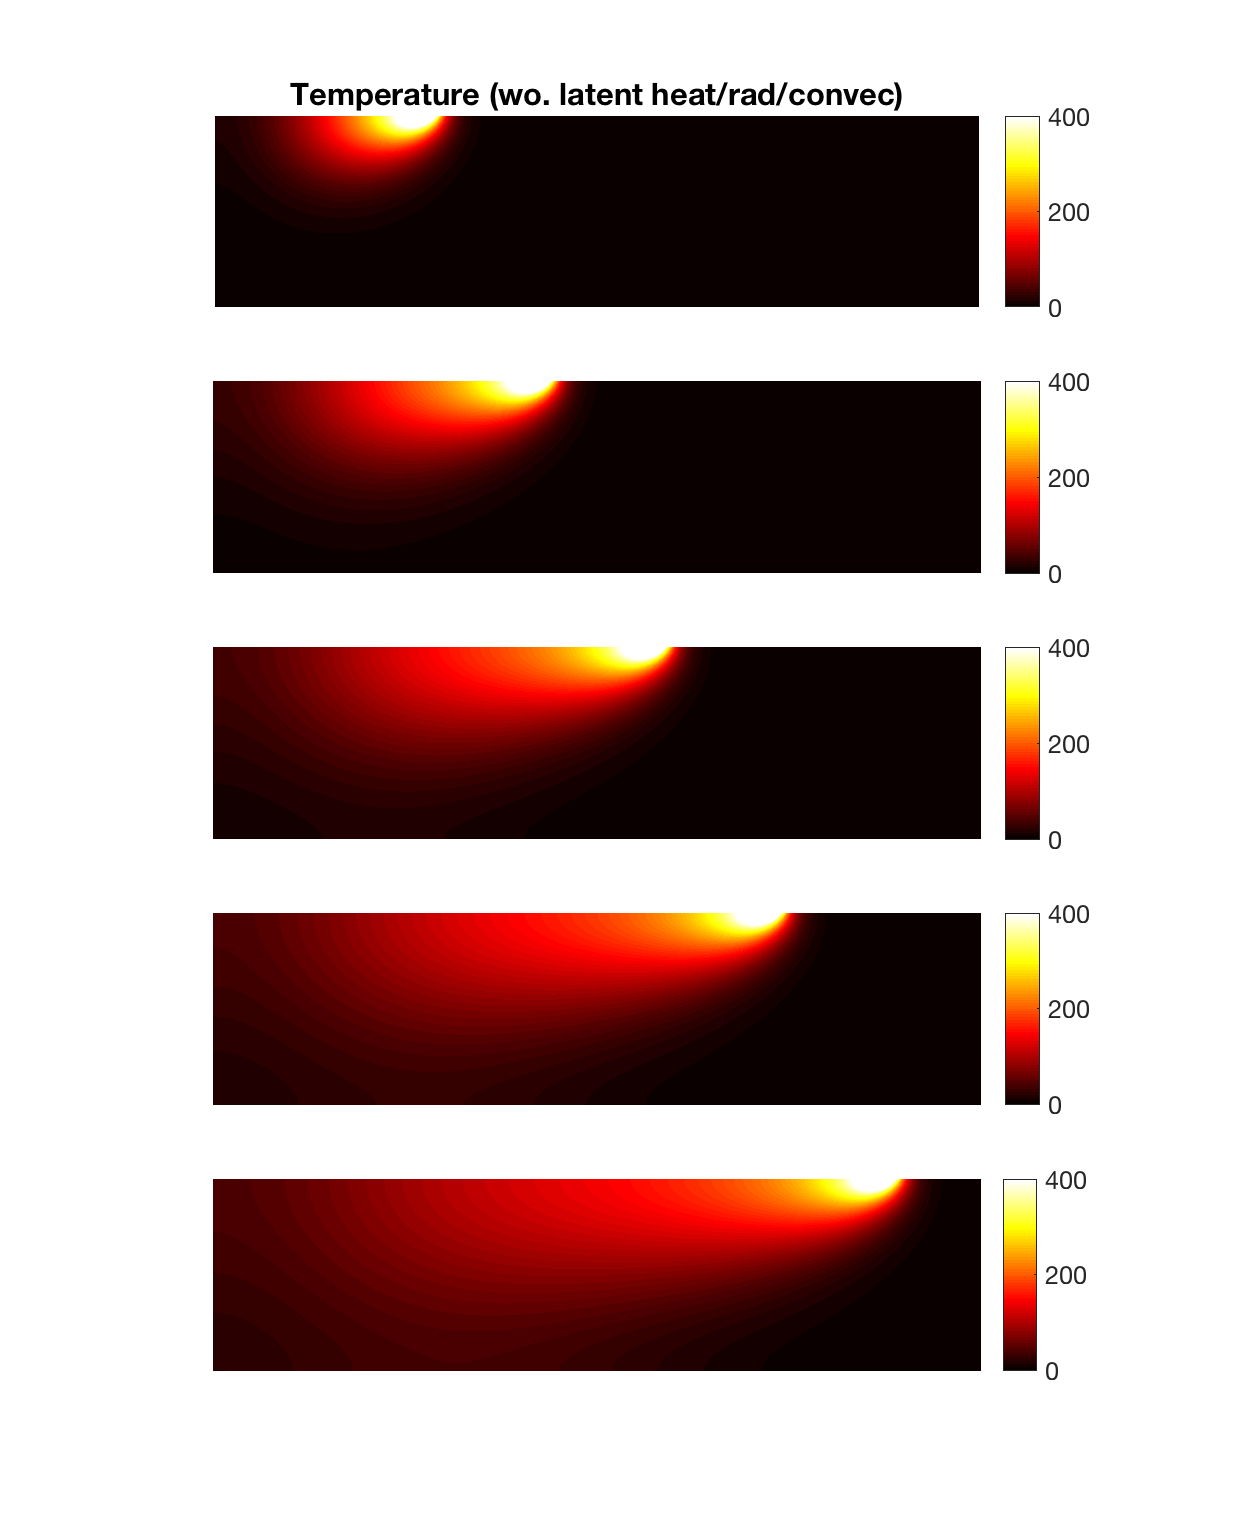
\includegraphics[width=0.45\textwidth]{./figures/temp_nlat_nrad.png}
     }
     \hfill
     \subfloat[$h_c$= 0.005, $\epsilon$ = 0.005\label{subfig-2:nlatwrad}]{%
       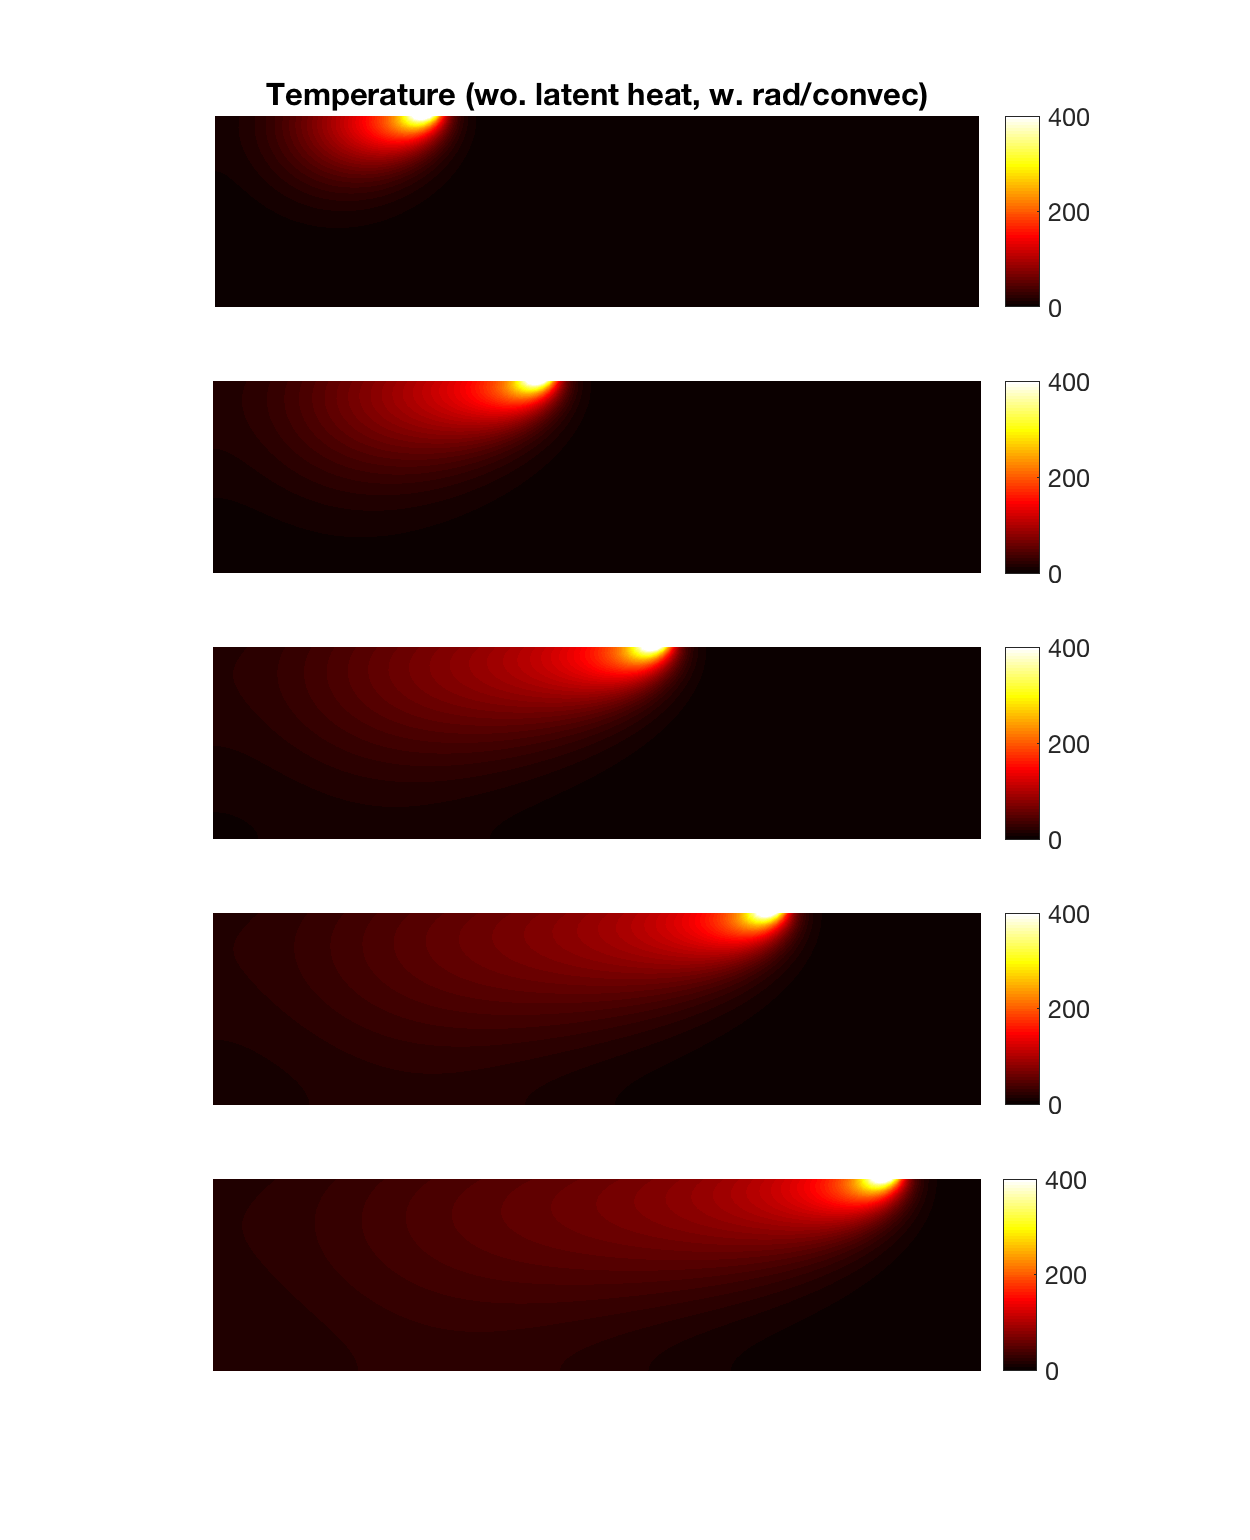
\includegraphics[width=0.45\textwidth]{./figures/temp_nlat_wrad.png}
     }
     \caption{Temperature distribution without latent heat.}
     \label{fig:nolatent}
   \end{figure}

\subsubsection{Self Convergence Study (with convection and radiation)}

Ground truth: dt = 0.00625, h = $ L_x/2048 $\\
Trial: dt = 0.025, 0.1, 0.4, 1.6; h =  $ L_x/1024, L_x/512, L_x/256, L_x/128 $

\begin{figure}[!ht]
     \subfloat[$L^2$ error \label{subfig-1:dummy}]{%
       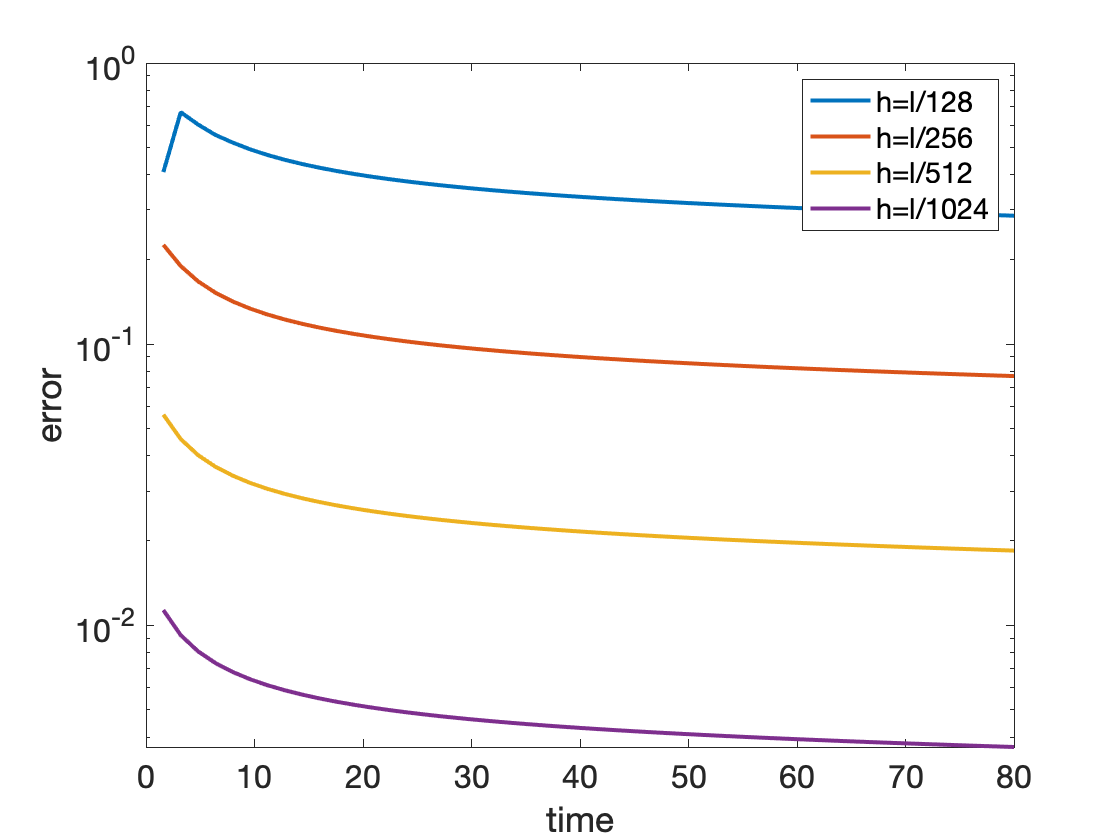
\includegraphics[width=0.45\textwidth]{./figures/self_convergence.png}
     }
     \hfill
     \subfloat[convergence order 2.076\label{subfig-2:dummy}]{%
       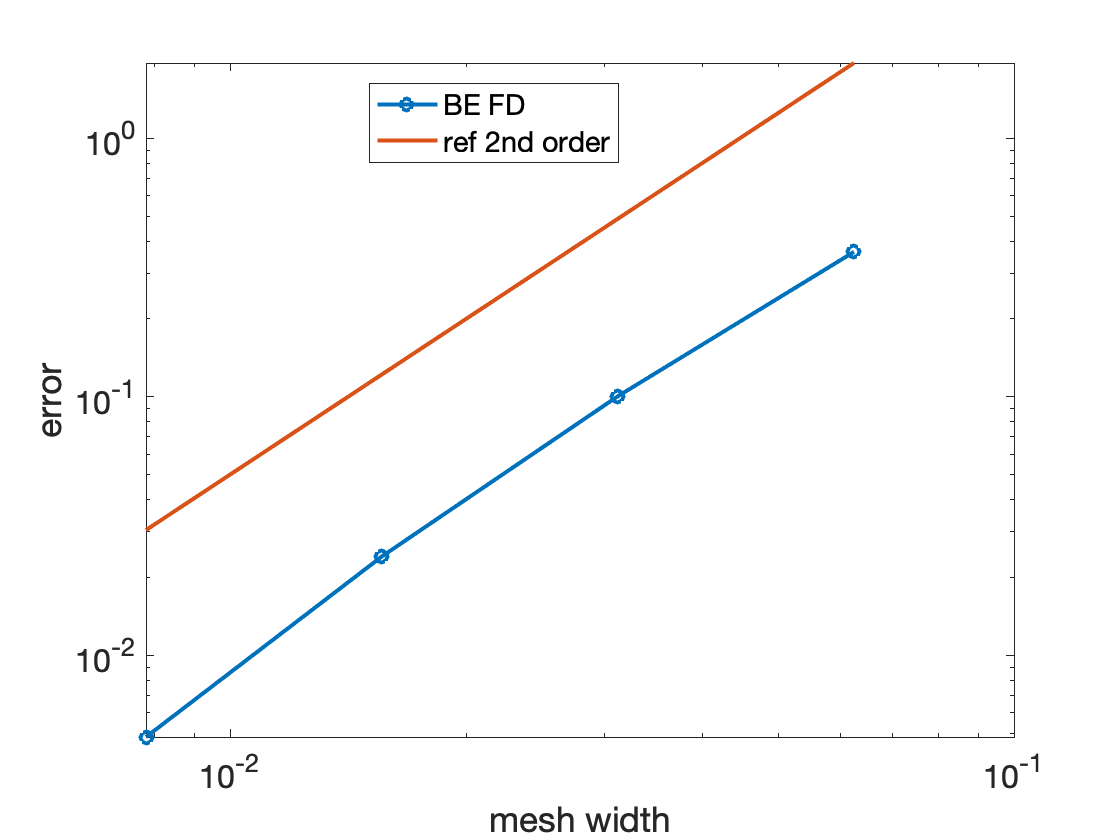
\includegraphics[width=0.45\textwidth]{./figures/Convergence_order.png}
     }
     \caption{Self convergence. }
     \label{fig:nolat_convergence}
   \end{figure}


\subsection{Latent heat term implicit-explicit}
Implicit: 
\begin{equation}
\frac{\partial   f_l(T)}{\partial t} = \frac{f_l^{n}(T)-f_l^{n-1}(T)}{\Delta t} 
\end{equation}
Explicit: 
\begin{equation}
f_l^{n}(T) =
\left\{
\begin{array}{cc}
1 & T^{n-1}>T_l \\
\frac{T^n-T_s}{T_l - T_s} & T_s \leq T^{n-1} \leq T_l \\
0 & T^{n-1} < T_s
\end{array}
\right.
\end{equation}

\begin{equation}
f_l^{n-1}(T) =
\left\{
\begin{array}{cc}
1 & T^{n-1}>T_l \\
\frac{T^{n-1}-T_s}{T_l - T_s} & T_s \leq T^{n-1} \leq T_l \\
0 & T^{n-1} < T_s
\end{array}
\right.
\end{equation}


\begin{equation}
\text{Latent heat term}=
\left\{
\begin{array}{cc}
0 & T^{n-1}>T_l \\
-\frac{L_m}{\Delta t}\frac{T^{n}-T^{n-1}}{T_l - T_s} & T_s \leq T^{n-1} \leq T_l \\
0 & T^{n-1} < T_s
\end{array}
\right.
\end{equation}
\\
\subsubsection{Test2}
Parameters: $L$=200, $T_s$=40, $T_l$=110\\

\begin{figure}[!ht]
     \subfloat[Without latent heat\label{subfig-1:nlat}]{%
       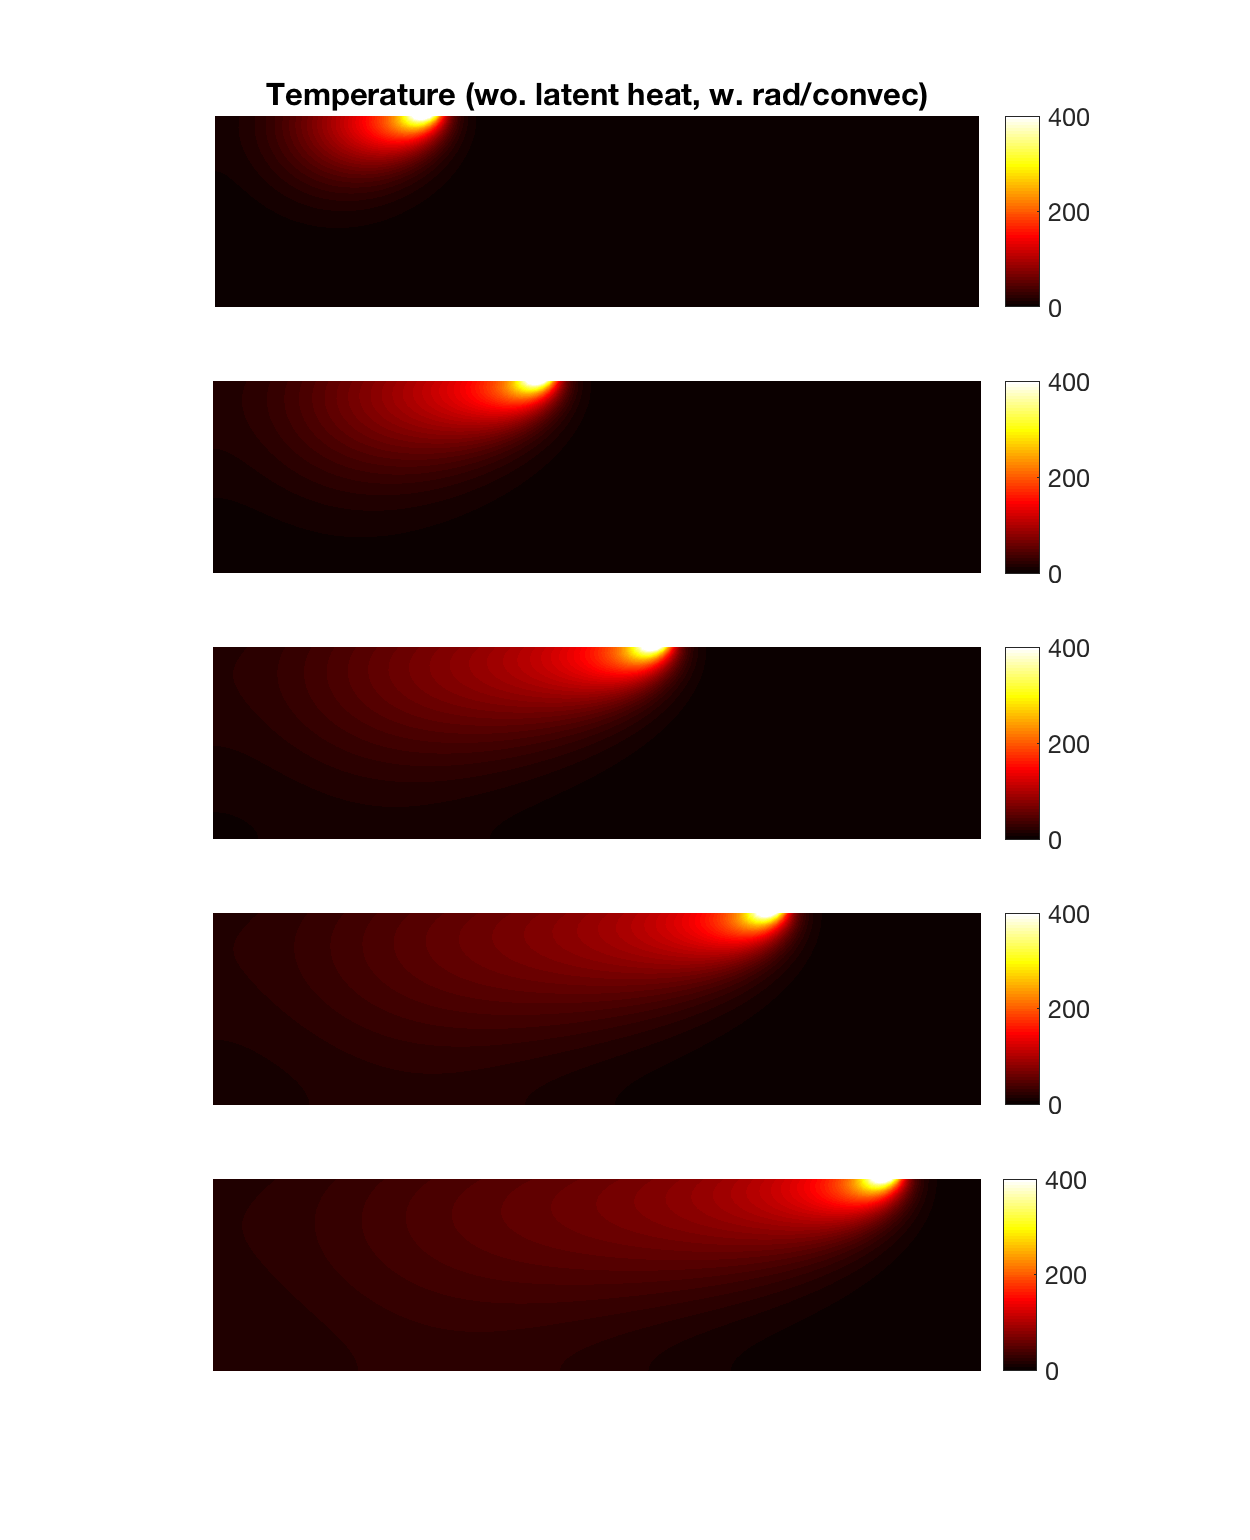
\includegraphics[width=0.45\textwidth]{./figures/temp_nlat_wrad.png}
     }
     \hfill
     \subfloat[With latent heat \label{subfig-2:lat}]{%
       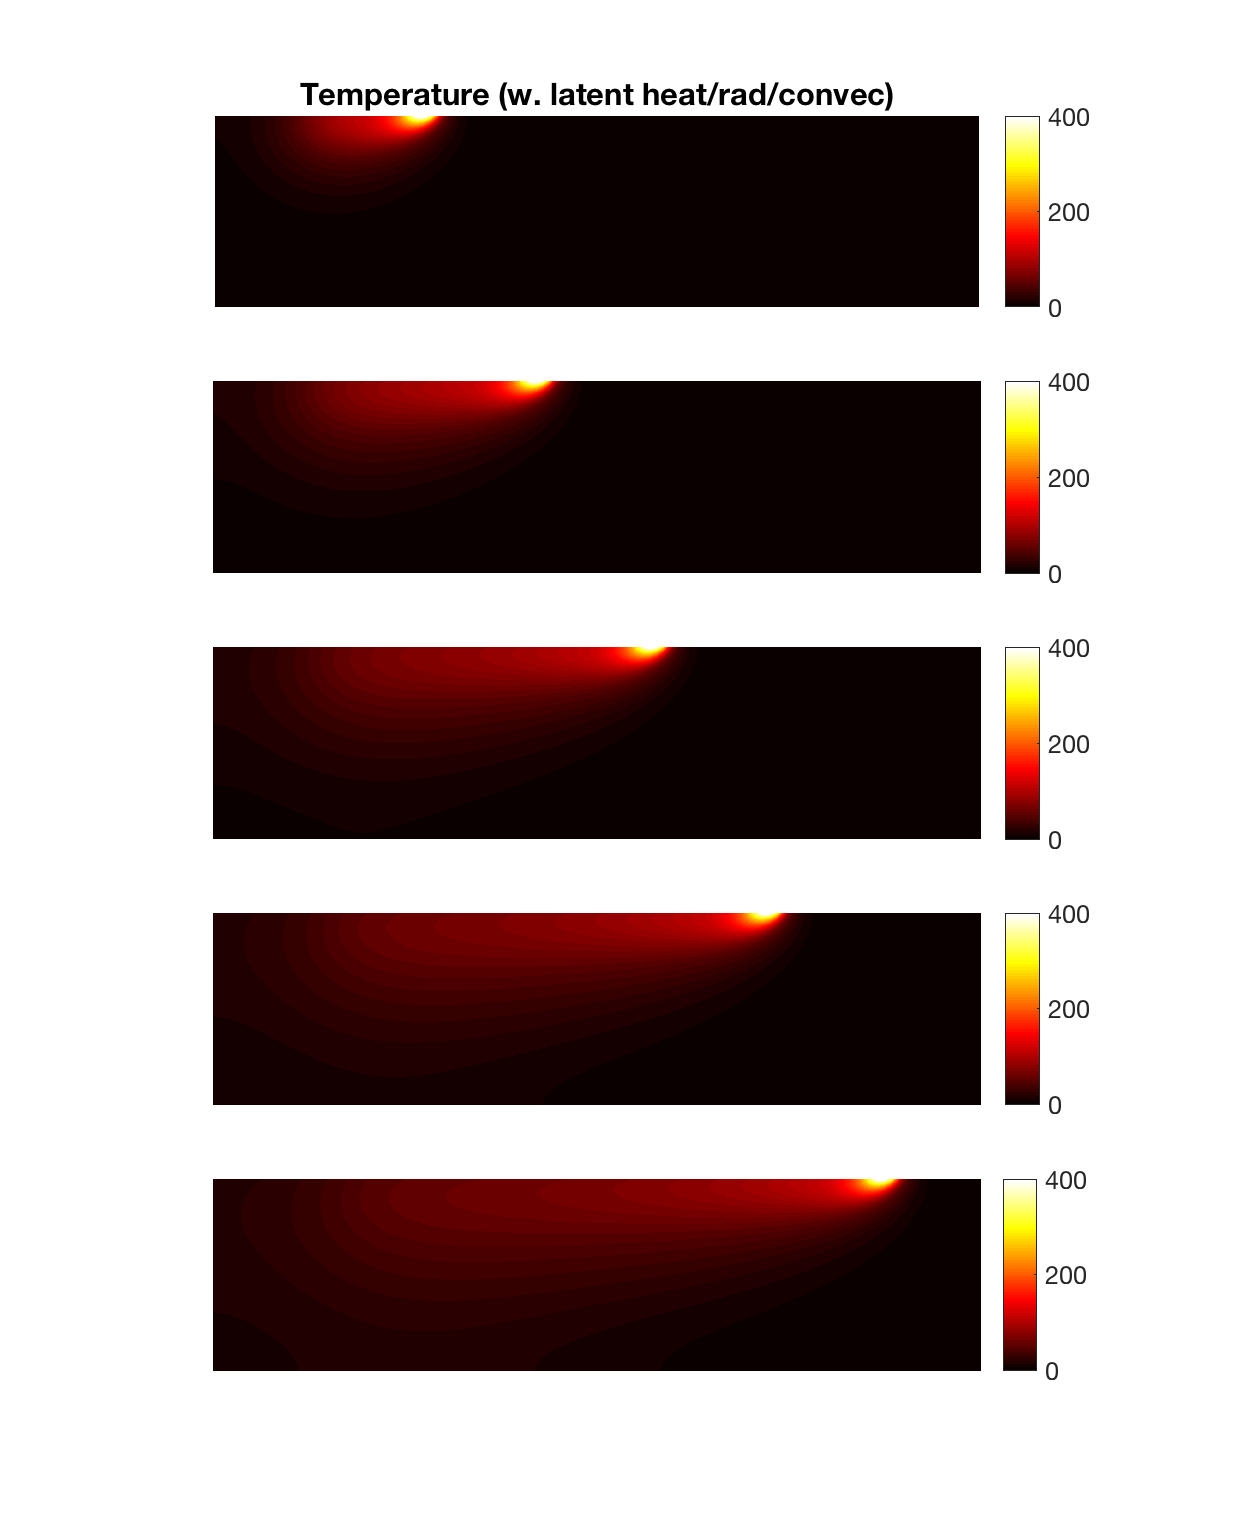
\includegraphics[width=0.45\textwidth]{./figures/temp_wlat_wrad.png}
     }
     \caption{Temperature distribution with and without latent heat. Surface cooling is included.}
     \label{fig:temp}
   \end{figure}


\begin{figure}[!ht]
     \subfloat[$L^2$ error \label{subfig-1:dummy}]{%
       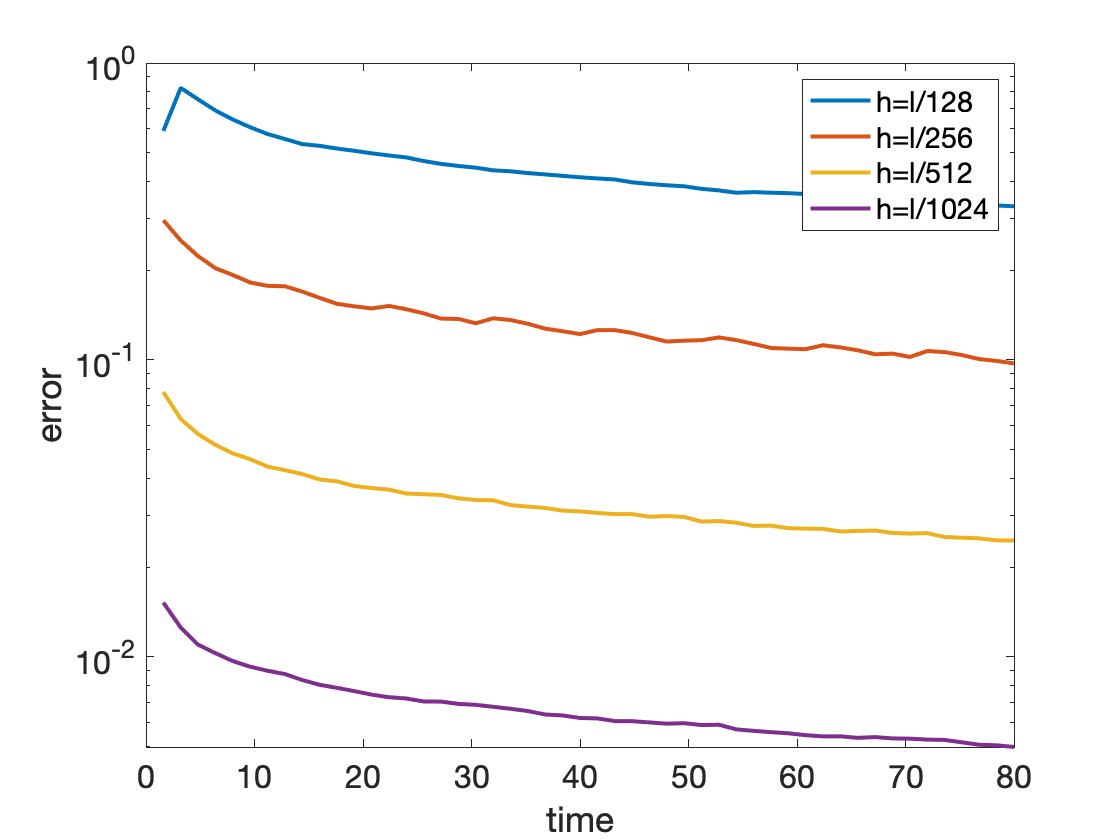
\includegraphics[width=0.45\textwidth]{./figures/self_lat.png}
     }
     \hfill
     \subfloat[convergence order\label{subfig-2:dummy}]{%
       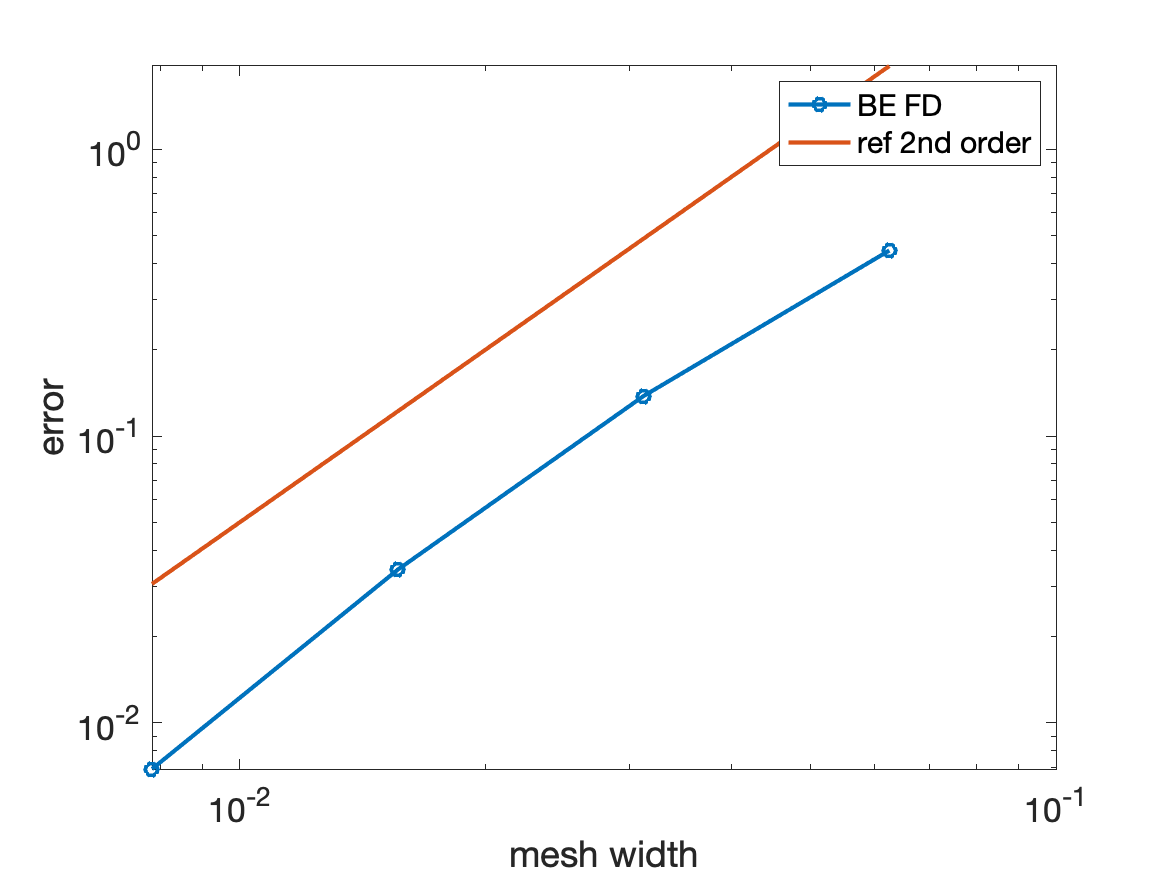
\includegraphics[width=0.45\textwidth]{./figures/convergence_lat.png}
     }
     \caption{Self convergence. }
     \label{fig:nolat_convergence}
   \end{figure}
GMRES solver (Tol = 1e-9):\\
For mesh width h =  $ L_x/1024, L_x/512, L_x/256, L_x/128 $\\
Iterations per time step without precondtioner: 58, 54, 48, 49, 50\\
Iterations per time step with precondtioner: 20, 17, 16,...      \ \        but took longer time to run

\newpage

\section{Microscopic model}

This model also makes the frozen temperature approximation \cite{Tourret2015,Echebarria2010,Plapp2007,Echebarria2004}:
\begin{align}
    & T(z,t) = T_0 + G(z-Rt),
\end{align}
where $T_0 = T_m - |m|c_{\infty}/k$. 

The compute set of phase-field equations are 
\begin{align}
\tau_{\phi} (\hat{n},z) \frac{\partial \phi}{\partial t} &= W^2_0 \left\{ \div{} [a_s(\hat{n})^2 \grad{} \phi] +  \partial_x \left( |\grad{} \phi|^2 a_s(\hat{n}) \frac{\partial a_s(\hat{n})}{\partial (\partial_x \phi)}  \right)  +
\partial_z \left( |\grad{} \phi|^2 a_s(\hat{n}) \frac{\partial a_s(\hat{n})}{\partial (\partial_z \phi)}  \right)  \right \}  \nonumber \\
& \quad + \phi - \phi^3 - \lambda (1-\phi^2)^2 \left(U + \frac{z-R t}{ l_T} \right),  \label{eq:micro_phi}\\
\tau_U \frac{\partial U}{\partial t} &= \div{} [D_l d(\phi) \grad{} U + \vec{j}_{at}] + [1+(1-k)U]\frac{1}{2}  \frac{\partial \phi}{\partial t}, \label{eq:micro_U}
\end{align}
where 
\begin{align}
U = \frac{1}{1-k} \left[ \frac{c/(c_{\infty}/k)}{(1-\phi)/2 + k(1+\phi)/2} \right], \quad d(\phi) = (1-\phi)/2 .
\end{align}
Other parameters and terms are defined as
\begin{align}
    & \tau_{\phi}(\hat{n},z) = \tau_0(a_s(\hat{n}))^2 \left[1-(1-k) \frac{(z-Rt)}{ l_T} \right] \\
	& \tau_U = \frac{1+k}{2} - \frac{1-k}{2}\phi \\
	& \vec{j}_{at} =  \frac{1}{2\sqrt{2}} W_0 [1+(1-k)U] \frac{\nabla \phi}{|\nabla \phi|} \frac{\partial \phi}{\partial t} \\
	& a_{s}(\hat{n}) = (1-3\delta)\left\{1+\frac{4 \delta}{1-3\delta}(\hat{n}_x^4 + \hat{n}_z^4) \right\} \\
    & \hat{n} =  \frac{\nabla \phi}{|\nabla \phi|} \\
    & l_T = \frac{|m|c_{\infty}(1/k-1)}{G} \\
    & \lambda =  \frac{5\sqrt{2}}{8}  \frac{W_0}{d_0} \\
    & d_0 = \frac{\Gamma}{|m|c_{\infty}(1/k-1)} = \frac{\gamma T_m/L}{|m|c_{\infty}(1/k-1)}  \\
    & \tau_0 =  \frac{0.6267\lambda W_0^2}{D_l}
\end{align}

\begin{table}
\centering
\begin{tabular}{l l c c }
\toprule
symbol & meaning & values & units \\
\midrule
$c_{\infty}|m|$ & shift in melting temperature &  1.0-2.0 & K \\
$k$ & interface solute partition coefficient & 0.1-0.3 &\\
$T_0$ & reference solidus temperature &  &\\
$T_m$ & melting temperature of pure material $A$ &  &\\
$l_T$ & thermal length &  & mm \\
$\gamma$ &  average surface tension &  & \\
$\delta$ & strength of the surface tension anisotropy  &  0.007 or 0.011 &\\
$\Gamma$ & Gibbs-Thompson coefficient & $6.4\times 10^{-8}$ & Km \\
$d_0$ & capillary length & $\approx 10^{-3}$  & $\mu$m \\
$G$ & thermal gradient & 10-300 & $\text{K} / \text{cm}$ \\
$R$ & pulling speed &  8-32 & $\mu \text{m} / \text{s}$ \\
$D_l$ & solute diffusion coefficient &$10^{-9}$ &  $\text{m}^2/\text{s}$ \\
$L$ & latent heat &  & \\
$W_0$ & interface thickness  & 40-90  & $d_0$ \\
$\Delta x$ & mesh size & 0.4-0.8 & $W_0$ \\
\bottomrule
\end{tabular}
\end{table}


The boundary conditions are periodic in the $x$-direction and no-flux in the $z$-direction.


\subsection{Micro model discretization}
\subsubsection{$\phi$-equation}
We first discretize the $\phi$-equation in \cref{eq:micro_phi}. The challenge is to discretize the anisotropic surface tension term. We will make a few simplications. First, note the anisotropic surface tension can be parametrized by $\theta \equiv \arctan(\phi_y / \phi_x)$, i.e., 
\begin{align}
& a_s(\theta)=  1 + \delta \cos(4 \theta) \\
& a_s'(\theta) = -4 \delta \sin(4\theta) 
\end{align}
By using some trigonometric identities (check), and $\cos(\theta) = \phi_x / |\grad{} \phi|$ and  $\sin(\theta) = \phi_y / |\grad{} \phi|$, we have
\begin{align}
& \cos(4\theta) = 1-8\cos^2(\theta) \sin^2(\theta) = 1- 8 \frac{ \phi_x^2 \phi_z^2 }{|\grad{} \phi|^4} \\
& \sin(4\theta) = 4 \sin(\theta) \cos(\theta) ( \cos^2(\theta) - \sin^2(\theta)) = 4 \frac{(\phi_x^3 \phi_z - \phi_x \phi_z^3 )}{|\grad{} \phi|^4}.
\end{align}
We can also write (see Appendix B of \cite{Tourret2015})
\begin{align}
& \partial_x \left( |\grad{} \phi|^2 a_s(\hat{n}) \frac{\partial a_s(\hat{n})}{\partial (\partial_x \phi)}  \right) = \partial_x (-a'_s(\theta) a_s(\theta) \partial_z \phi ) \\
& \partial_z \left( |\grad{} \phi|^2 a_s(\hat{n}) \frac{\partial a_s(\hat{n})}{\partial (\partial_z \phi)}  \right) = 
\partial_z (a'_s(\theta) a_s(\theta) \partial_x \phi).
\end{align}
Therefore,
\begin{align}
 & \div{} [a_s(\hat{n})^2 \grad{} \phi] +  \partial_x \left( |\grad{} \phi|^2 a_s(\hat{n}) \frac{\partial a_s(\hat{n})}{\partial (\partial_x \phi)}  \right)  +
\partial_z \left( |\grad{} \phi|^2 a_s(\hat{n}) \frac{\partial a_s(\hat{n})}{\partial (\partial_z \phi)}  \right) \nonumber \\
= &  \  \partial_x  \underbrace{ \left[ a_s^2(\theta) \partial_x \phi - a'_s(\theta) a_s(\theta) \partial_z \phi \right]}_{=: F} + 
\partial_z \underbrace{ \left[ a_s^2(\theta) \partial_z \phi + a'_s(\theta) a_s(\theta) \partial_x \phi \right]}_{=: J}  
\label{eq:aniso_surf2}
\end{align}

We define $\phi(i,j)$ on the cell nodes. Therefore, \cref{eq:aniso_surf2} is discretized as
\begin{equation}
\frac{F(i+1/2, j) - F(i-1/2,j)}{\Delta x} + \frac{J(i,j+1/2)-J(i,j-1/2)}{\Delta z}
\end{equation}
Note $F,J$ are defined on cell edges. For example, to evaluate $F(i+\frac{1}{2},j)$, we need to evaluate
\begin{align}
& a_s(\theta) \bigg|_{i+1/2,j} = \left( 1-3\delta + 4\delta  \frac{\phi_x^4 +  \phi_z^4}{|\grad{} \phi|^4} \right)\bigg|_{i+1/2,j} \\
& a'_s(\theta) \bigg|_{i+1/2,j} = -16\delta  \frac{(\phi_x^3 \phi_z- \phi_x \phi_z^3 )}{|\grad{} \phi|^4} \bigg|_{i+1/2,j}\\
& \partial_x \phi \bigg|_{i+1/2,j} = \frac{\phi_{i+1,j}-\phi_{i,j}}{\Delta x} \\
& \partial_z \phi \bigg|_{i+1/2,j}  = \frac{1}{4} \left( \frac{\phi_{i,j+1}-\phi_{i,j}}{\Delta z} +  \frac{\phi_{i+1,j+1}-\phi_{i+1,j}}{\Delta z} +  \frac{\phi_{i,j}-\phi_{i,j-1}}{\Delta z}  +  \frac{\phi_{i+1,j}-\phi_{i+1,j}}{\Delta z} \right)
\end{align}
Note evaluating $\partial_z \phi |_{i+1/2,j}$ requires averaging nearby cells.  Please work out the details for $F(i-1/2,j)$, $J(i,j+1/2)$ and $J(i,j-1/2)$. Many of them are redundant. I think you only need 
$\partial_x \phi |_{i,j+1/2}$ and $\partial_z \phi |_{i,j+1/2}$.


\yxb{Note that you need both $a_s(\grad{}\phi_{i\pm 1/2, j\pm 1/2} )$ for $a_s(\hat{n})$ on the right-hand-side and $a_s(\grad{}\phi_{i, j} )$ for $\tau_{\phi}(\hat{n},z)$ on the left-hand-side.}


Once we discretize \cref{eq:aniso_surf2}, the rest is straightforward. Please fill in the details.

\subsubsection{Divide-by-zero in anisotropy}
There are two ways to treat the numerical issue of divide-by-zero in computing $a_s(\theta)$.
\begin{enumerate}
\item On page 66 of \cite{Provatas2010}, when $|\grad{}\phi(i,j)|^{4} \leq \epsilon $, say $\epsilon = 10^{-8}$,
\begin{align*}
a_s(\hat{n}) &= 1-3\delta, \\
a'_s(\hat{n}) &= 0.
\end{align*}

\item We can also regularize 
\end{enumerate}




\subsubsection{Divide-by-zero in anisotropy}
There are two ways to treat the numerical issue of divide-by-zero in computing $a_s(\theta)$.
\begin{enumerate}
\item On page 66 of \cite{Provatas2010}, when $|\grad{}\phi(i,j)|^{4} \leq \epsilon $, say $\epsilon = 10^{-8}$,
\begin{align*}
a_s(\hat{n}) &= 1-3\delta, \\
a'_s(\hat{n}) &= 0.
\end{align*}

\item We can also regularize 
\end{enumerate}


\subsubsection{$U$-equation}
\begin{itemize}
\item A routine that takes in edge-centered vector data and outputs the divergence at cell nodes, i.e.,
\begin{equation}
\div{} \B{u} = \frac{u_{i+1/2,j} - u_{i-1/2,j}}{\Delta x} +  \frac{v_{i, j+1/2} - v_{i,j-1/2}}{\Delta z}
\end{equation}

\item we need the following terms at $(i+1/2,j)$ and $(i,j+1/2)$
\begin{align}
& [(1-\phi) U_x]_{i+1/2,j} = \left( 1- \frac{\phi_{i+1,j} + \phi_{i,j}}{2} \right) \frac{U_{i+1,j}-U_{i,j}}{\Delta x}\\
& [(1-\phi) U_z]_{i,j+1/2} = ?
\end{align}

\item Similarly, for the anti-trapping flux $\vec{j}_{at}$, we need
\begin{align}
\left[ [1+(1-k)U]  \frac{\phi_x}{ |\grad{} \phi | } \frac{\partial \phi}{\partial t}  \right]_{i+1/2,j} = ? \\
\left[ [1+(1-k)U]  \frac{\phi_y}{ |\grad{} \phi | } \frac{\partial \phi}{\partial t}  \right]_{i,j+1/2} = ? \\
\end{align}
\end{itemize}

\yxb{The bottom line with finite difference is that: whenever the quantity is not defined on the target grid points, you just average nearby cell data.}

\yxb{I strongly recommend you read the appendices of \cite{Tourret2015}, and page 65, page 101-102 of \cite{Provatas2010}. }




\bibliographystyle{unsrt}
\bibliography{Directional-Solidification.bib}


%%%%%%%%%%%%%%%%%%%%%%%%%%%%%%%%%%%%%%%%%%%%%%%

\end{document}
